\documentclass[fleqn]{jbook}
\usepackage{physpub}

\begin{document}

\begin{question}{教育 数学}{}

\begin{subquestions}
\SubQuestion
  時間$t$の関数$y(t)$に関する非線型微分方程式
%
  \begin{equation}
  \Deriver{^2y}{t^2} + y = \eps y^3 \eqname{1-1}
  \end{equation}
%
  を、$t=0$における初期条件
%
  \begin{equation}
  y=1 \hspace{15mm} \Deriver{y}{t}=0 \eqname{1-2}
  \end{equation}
%
  のもとで考察する。ただし、$\varepsilon$は微小な正の定数とする。
  必要なら、$i$を虚数単位として、次の恒等式を用いよ。
%
  \begin{equation}
  (\cos\theta+i\sin\theta)^3= \cos{3\theta}+i\sin{3\theta} \eqname{1-3}
  \end{equation}
%
  \begin{subsubquestions}
  \SubSubQuestion
    $y$を$\eps$に関し、
%
    \begin{equation}
    y(t;\eps) = \sum^{\infty}_{n=0} \eps^n y_n(t) \eqname{1-4}
    \end{equation}
%
    と展開するとき、$y_{0},y_{1}$に対する方程式および初期条件を求めよ。

  \SubSubQuestion
    前問の各方程式を解き、$y_{0},y_{1}$を求めよ。

  \SubSubQuestion
    前問の結果より、この展開にもとづく解の適否を、$t$が大きくなった
    場合について論ぜよ。
  \end{subsubquestions}



\SubQuestion
  3行2列の実行列 $A$ を
%
  \begin{equation}
    A = U \Lambda \Trans{V}   \eqname{2-1}
  \end{equation}
%
  のように分解することを考える。ただしTは転置行列を表し、
  $U,\Lambda,V$ はそれぞれ3行2列、2行2列、2行2列の実行列で、以下の通りである。
%
  \begin{equation}
    \Trans{V} V = V \Trans{V} = \Trans{U} U%
    = \begin{pmatrix} 1 & 0 \\ 0 & 1 \end{pmatrix}%
    \equiv I \hspace{15mm}%
    \Lambda = \begin{pmatrix} \lambda_1 & 0 \\ 0 & \lambda_2 \end{pmatrix}%
    \hspace{5mm} \lambda_1 \geq \lambda_2 \geq 0%
    \eqname{2-2}
  \end{equation}

  \begin{subsubquestions}
  \SubSubQuestion
    式\eqhref{2-1}のように分解ができたとして、行列 $\Trans{A}A$ の
    すべての固有値とそれに対応する固有ベクトルとを
    $U, \Lambda, V, \lambda_1, \lambda_2$ を用いて表せ。
    必要なら次の単位ベクトルを用いてよい。
%
    \[%
      \vec{e}_1 = \begin{pmatrix} 1 \\ 0 \end{pmatrix} \hspace{10mm} %
      \vec{e}_2 = \begin{pmatrix} 0 \\ 1 \end{pmatrix} %
    \]
%

  \SubSubQuestion
    \parbox[t]{100mm}{
    行列 $A$が右のように与えれるとき、
    $ \Trans{A}A$ の固有値および長さ$1$の固有ベクトルを
    すべて求めよ。ただし各固有ベクトルの第1要素は非負とする。
    }\parbox[t]{50mm}{\vspace*{-5mm}
    \[ A = \frac{1}{2}\begin{pmatrix}%
      3+\sqrt{2} & 3-\sqrt{2} \\
      3-\sqrt{2} & 3+\sqrt{2} \\
      3\sqrt{2}  & 3\sqrt{2}  \end{pmatrix} \]
    }

  \SubSubQuestion
    前問の行列$A$に対して式\eqhref{2-1}を満たす
    $U, \Lambda, V$ を求めよ。ただし$V$ の第1行の各要素は非負とする。

  \end{subsubquestions}



\SubQuestion
  \parbox[t]{100mm}{
  床一面に引かれた間隔$a$の平行線に上から長さ$\ell(\geq a)$の棒を
  落としたとき、棒が平行線と交わる確率$P(\ell)$を以下の手順に
  したがって求めよ。

  \begin{subsubquestions}
  \SubSubQuestion
    棒の一端が平行線から$x$の距離$(0\leq x \leq a/2)$にあるとき、
    棒が平行線と交わる確率$p(x)$を求めよ。ただし、棒の方位角は
    床面内で一様に分布するものとする。また、棒の太さは無視する。

  \SubSubQuestion
    $x$が$[0,a/2]$の区間内で一様に分布するとして、$P(\ell)$を求めよ。

  \end{subsubquestions}

  }\parbox[t]{55mm}{\vspace*{-5mm}
  \begin{center}
    \mbox{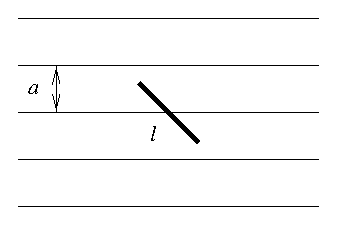
\includegraphics[clip]{1995math-1.eps}}
  \end{center}}



\end{subquestions}
\end{question}
\begin{answer}{教育 数学}{}

\begin{subanswers}
\SubAnswer

  \begin{subsubanswers}
  \SubSubAnswer
    求めるべきものは $\eps$ の0次と1次に関する項のみなので
    式\eqhref{1-4}の展開は$\eps$の1次までで十分である。
%
    \begin{equation}
      y(t;\eps) = y_0(t) + \eps y_1(t) + O(\eps^2) \eqname{1-5}
    \end{equation}
%
    この式を微分方程式\eqhref{1-1}と初期条件式\eqhref{1-2}に
    それぞれ代入して$\eps$の項で整理すると以下の式が得られる。
%
    \begin{eqnarray}
      \ddot{y}_0(t) + y_0(t) &=& 0           \eqname{1-6} \\
      \ddot{y}_1(t) + y_1(t) &=& y_0(t)^3    \eqname{1-7}
    \end{eqnarray}
    \begin{equation}
      y_0(0)=1 \hspace{10mm} \dot{y}_0(0)=0 \hspace{10mm}
      y_1(0)=0 \hspace{10mm} \dot{y}_1(0)=0 \eqname{1-8}
    \end{equation}
%   
    これが求める$y_0,y_1$に対する方程式と初期条件である。


  \SubSubAnswer
    $y_0(t)$ は微分方程式\eqhref{1-6}と初期条件\eqhref{1-8}より明らかに
%
    \[ y_0(t) = \cos{t} \]
%
    である。続いて$y_1(t)$は微分方程式\eqhref{1-7}より
%
    \begin{equation}
      \ddot{y}_1(t) + y_1(t) = \cos^3{t} = \frac{3}{4}\cos{t} + \frac{1}{4}\cos{3t}  \eqname{1-9}
    \end{equation}
%   
    である。この非斉次の線形微分方程式を解法は、(a)非斉次項のない
    斉次の方程式の一般解を求め、(b)非斉次項のある方程式の特殊解を
    求めて、両者の和をとることである。\\
%
    (a)は明らかに
    \[ y_1(t) = C_1\cos{t} + C_2\sin{t} \]
    である。$C_1,C_2$は後で定める定数である。\\
    (b)は非斉次項が2つあるのでその個々の項だけの非斉次方程式の特殊
    解を適当に探す。すなわち、
%
    \begin{eqnarray*}
      \ddot{y}_1(t) + y_1(t) &=& \frac{3}{4}\cos{t}\quad\Longrightarrow y_1(t) = \frac{3}{8}t\sin{t} \\
      \ddot{y}_1(t) + y_1(t) &=& \frac{1}{4}\cos{3t}\;\;\Longrightarrow y_1(t) = -\frac{1}{32}\cos{3t}
    \end{eqnarray*}
%
    が得られこの和が(b)の特殊解である。\\
    よって $y_1(t)$ の解は初期条件\eqhref{1-8}を考慮して
%
    \[ y_1(t) = \frac{1}{32}\cos{t} - \frac{1}{32}\cos{3t} + \frac{3}{8}t\sin{t} \]
%
    である。


  \SubSubAnswer
    前問で得られた $y_1(t)$ の解の振動の振幅は$t$の増大と共に激しく
    なる。この傾向は式\eqhref{1-4}の展開の後続の項でもより顕著となる
    ので、展開は$t$が十分大きければ収束しない。よってこの展開は
    妥当ではない。

  \end{subsubanswers}

  
\SubAnswer
  \begin{subsubanswers}

  \SubSubAnswer
    式\eqhref{2-1}の表式と式\eqhref{2-2}の定義により
%
    \[ \Trans{A}A = \Trans{(U\Lambda\Trans{V})}(U\Lambda\Trans{V}) = %
       (V \Trans{\Lambda} \Trans{U} ) U \Lambda \Trans{V} = %
       V \Lambda^2 \Trans{V} \]
%
    であることがわかる。\\
%
    指標$i$を$i=1,2$として、$\Trans{A}A$ の2つの固有値を
    $\alpha_i$、固有ベクトルを $\vec{u}_i$ と表すと前式より
%
    \[ V \Lambda^2 \Trans{V} \vec{u}_i = \alpha_i \vec{u}_i \]
%
    となる。この両辺に左から $\Trans{V}$をかけると、$\Trans{V}V=I$
    より
%
    \[ \Lambda^2\Trans{V}\vec{u}_i = \alpha_i\Trans{V}\vec{u}_i \]
%
    すなわち、$\Trans{V}\vec{u}_i$ は $\Lambda^2$ の固有値 $\alpha_i$
    の固有ベクトルである。ところで、
%
    \[ \Lambda^2 = \begin{pmatrix}
                       \lambda_1^2 & 0 \\%
                       0 & \lambda_2^2 \end{pmatrix} \]
%
    であるから、その固有値は明らかに $\lambda_1^2$ および $\lambda_2^2$
    であり、対応する固有ベクトルはそれぞれ $\vec{e}_1$、$\vec{e}_2$ 
    である。

    以上のことより $\Trans{A}A$ の固有値は $\lambda_1^2$ および
    $\lambda_2^2$ であり、対応する固有ベクトルは、
    $\Trans{V}\vec{u}_i = \vec{e}_i$ からそれぞれ
    $\vec{u}_1 = c_1 V \vec{e}_1$、$\vec{u}_2 = c_2 V \vec{e}_2$
    である。($c_1,c_2$は定数)


  \SubSubAnswer
    そのまま計算して
%
    \[ \Trans{A}A = \frac{1}{2}\begin{pmatrix}%
      3+\sqrt{2} &3-\sqrt{2} &3\sqrt{2}  \\
      3-\sqrt{2} &3+\sqrt{2} &3\sqrt{2}  
     \end{pmatrix}%
     \frac{1}{2}\begin{pmatrix}%
      3+\sqrt{2} &3-\sqrt{2}  \\
      3-\sqrt{2} &3+\sqrt{2}  \\
      3\sqrt{2}  &3\sqrt{2}   
     \end{pmatrix}%
     = \begin{pmatrix} 10 & 8 \\ 8 & 10 \end{pmatrix} \]
%
     この固有値 $\alpha_i$ は ${\rm det}(\Trans{A}A-\alpha_i I)=0$ より
%
     \[ \left| \begin{matrix}%
      10-\alpha_i & 8 \\
      8 & 10 - \alpha_i
     \end{matrix} \right|%
     = \alpha_i^2 - 20\alpha_i + 36 = 0 %
     \hspace{10mm} \alpha_1 = 2,\,\,\alpha_2 = 18 \]
%
     固有ベクトル $\vec{u}_i$ は、長さが1、第1成分が非負の条件より

     \[ \vec{u}_1 = \frac{1}{\sqrt{2}}%
        \begin{pmatrix} 1 \\  1 \end{pmatrix} \hspace{20mm}%
        \vec{u}_2 = \frac{1}{\sqrt{2}}%
        \begin{pmatrix} 1 \\ -1 \end{pmatrix} \]
%
    となる。


  \SubSubAnswer
    $\lambda_i^2 = \alpha_i,\,\,\lambda_1 \geq \lambda_2$ であるので
    前問の結果より $\lambda_1=3\sqrt{2},\,\,\lambda_2=\sqrt{2}$ となる。
    よって、
%
    \[ \Lambda = \begin{pmatrix}%
        3\sqrt{2} & 0 \\
        0 & \sqrt{2}  \end{pmatrix} \]
%
    次に、 $\vec{u}_i = V \vec{e}_i$ であるので
%
    \[ V = \frac{1}{\sqrt{2}} \begin{pmatrix}%
        1 &  1 \\
        1 & -1 \end{pmatrix} \]
%
    最後に $U = AV\Lambda^{-1}$ であるので
%
    \[ U = \frac{1}{2}\begin{pmatrix}%
          3+\sqrt{2} & 3-\sqrt{2} \\
          3-\sqrt{2} & 3+\sqrt{2} \\
          3\sqrt{2}  & 3\sqrt{2}  \end{pmatrix}%
        \frac{1}{\sqrt{2}}\begin{pmatrix}
          1 &  1 \\
          1 & -1 \end{pmatrix}%
        \frac{1}{6}\begin{pmatrix}%
          \sqrt{2} & 0 \\
          0 & 3\sqrt{2} \end{pmatrix}%
        = \frac{1}{2}\begin{pmatrix}
           1 &  \sqrt{2} \\
           1 & -\sqrt{2} \\
          \sqrt{2} & 0 \end{pmatrix} \]
%
    と求まる。
  \end{subsubanswers}

\SubAnswer
  \begin{subsubanswers}
  \SubSubAnswer
    \parbox[t]{85mm}{
    初めに棒の一端が床に着地し、任意の方向に倒れると考えても一般性は
    失われない。\\
%
    倒れた棒が床の線と交わるには、棒が右図のマスクした領域の向きに
    倒れた場合である。右図でこの諸量を定義する。
%
    $x$を固定した場合の棒の線と交わる確率 $p(x)$ は明らかに
%
    \[ p(x) = \frac{2\theta_1+2\theta_2}{2\pi} = %
              \frac{ \theta_1+ \theta_2}{\pi} \]
%
    である。なお変数の定義から以下の式が成り立っている。
%
    \[ \theta_1 = \arccos\frac{x}{\ell} \hspace{15mm} %
       \theta_2 = \arccos\frac{y}{\ell} \]
%
    }\parbox[t]{70mm}{\vspace*{-10mm}
    \begin{center}
      \mbox{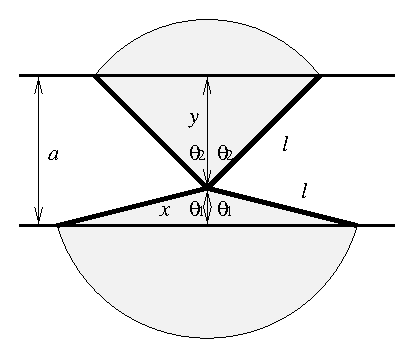
\includegraphics[clip]{1995math-2.eps}}
    \end{center}}

  \SubSubAnswer
    2本の平行線の中点に関して床は上下対称なので、求める確率は
    棒の着地点$x$を$[0,a/2]$の範囲に限定して考えて差し支えない。\\
%
    棒が線と交わる確率$P(\ell)$は、前問で得られた結果を規格化に
    注意して$x$で積分すれば求まる。すなわち
%
    \[ P(\ell) = \frac{1}{a/2} \Dint{0}{a/2}{\d{x}} p(x)%
               = \frac{2}{a\pi} \Bigl[%
                     \Dint{0}{a/2}{\d{x}} \theta_1%
                   + \Dint{0}{a/2}{\d{x}} \theta_2%
                  \Bigr] \]
%
    この右辺第2項で$y=a-x$の変数変換を行い、$\theta_1,\theta_2$を
    それぞれ$x,y$で表すと
%
    \[ P(\ell) = \frac{2}{a\pi} \Bigl[%
                     \Dint{0}{a/2}{\d{x}} \arccos\frac{x}{\ell}%
                   + \Dint{a/2}{a}{\d{y}} \arccos\frac{y}{\ell}
                     \Bigr]
\]
%
    となるがこの右辺第2項の被積分関数は右辺第1項のそれとまったく
    同じである。よって2つの積分をまとめて
%
    \[ P(\ell) = \frac{2}{a\pi} \Dint{0}{a}{\d{x}} \arccos\frac{x}{\ell} \]
%
    とすることができる。さらに$x=\ell\cos\theta$と変数変換してこの積分
    を計算する。
%
    \begin{eqnarray*}
      P(\ell) &=& -\frac{2\ell}{a\pi} \Dint{\arccos{(0)}}{\arccos{(a/\ell)}}{\d{\theta}} \theta\sin\theta%
               = \frac{2\ell}{a\pi} \Bigl[ \theta\cos\theta-\sin\theta \Bigr]_{\nsub{\arccos{(0)}}}^{\nsub{\arccos{(a/\ell)}}} \\
              &=& \frac{2\ell}{a\pi} \Bigl( \frac{a}{\ell} \arccos{\frac{a}{\ell}} - \frac{\sqrt{\ell^2-a^2}}{\ell} + 1 \Bigl) %
               =  \frac{2}{\pi} \Bigl( \arccos{\frac{a}{\ell}} - \frac{\sqrt{\ell^2-a^2} - \ell}{a} \Bigl)
    \end{eqnarray*}
%
    これが求める確率である。なお$a\to0$または$\ell\to\infty$の極限に
    おいてこの確率は確かに$1$になる。

  \end{subsubanswers}

\end{subanswers}
\end{answer}


\end{document}
